\documentclass[9pt,twocolumn,twoside]{pnas-new}
% Use the lineno option to display guide line numbers if required.

\templatetype{pnasresearcharticle} % Choose template 
% {pnasresearcharticle} = Template for a two-column research article
% {pnasmathematics} %= Template for a one-column mathematics article
% {pnasinvited} %= Template for a PNAS invited submission

\usepackage{epsfig}
\usepackage{verbatim}	 % for block comments \begin{comment} \end{comment}
\usepackage{amssymb}
% \usepackage{bbold}
\usepackage{bm}
\usepackage{amsmath}
\usepackage{psfrag}
\bibliographystyle{apsrev}
\usepackage{color}
% \usepackage{ulem}
%\usepackage[latin1]{inputenc}
%\usepackage[english]{babel}
\usepackage{graphicx}
\usepackage{amscd}
\usepackage{eucal}
\usepackage{bm}
%\usepackage{pslatex}
\usepackage{hyperref}
\usepackage{lipsum}
\usepackage{mathtools}
\usepackage{multirow}

\title{The K-player: some authors beat the power law}

% Use letters for affiliations, numbers to show equal authorship (if applicable) and to indicate the corresponding author
\author[a,b,1]{R. Delabays}
\author[a,c]{M. Tyloo} 

\affil[a]{School of Engineering, University of Applied Sciences of Western Switzerland HES-SO CH-1951 Sion, Switzerland.}
\affil[b]{Automatic Control Laboratory, Swiss Federal Institute of Technology (ETH) Z\"urich,  Switzerland.}
\affil[c]{Institute of Physics, EPF Lausanne, CH-1015 Lausanne, Switzerland.}

% Please give the surname of the lead author for the running footer
\leadauthor{Delabays} 

% Please add here a significance statement to explain the relevance of your work
\significancestatement{Authors must submit a 120-word maximum statement about the significance of their research paper written at a level understandable to an undergraduate educated scientist outside their field of speciality. The primary goal of the Significance Statement is to explain the relevance of the work in broad context to a broad readership. The Significance Statement appears in the paper itself and is required for all research papers.}

% Please include corresponding author, author contribution and author declaration information
\authorcontributions{Please provide details of author contributions here.}
\authordeclaration{Please declare any conflict of interest here.}
\equalauthors{\textsuperscript{1}A.O.(Author One) and A.T. (Author Two) contributed equally to this work (remove if not applicable).}
\correspondingauthor{\textsuperscript{1}To whom correspondence should be addressed. E-mail: author.two\@email.com}

% Keywords are not mandatory, but authors are strongly encouraged to provide them. If provided, please include two to five keywords, separated by the pipe symbol, e.g:
\keywords{Keyword 1 $|$ Keyword 2 $|$ Keyword 3 $|$ ...} 


%%\documentclass[aps,prb,floatfix,showpacs,preprint]{revtex4}
%\documentclass[aps,prl,floatfix,twocolumn]{revtex4-1}


\begin{abstract}
 \textcolor{red}{\lipsum[1]}
\end{abstract}

\dates{\today}

\begin{document}

\maketitle
\thispagestyle{firststyle}
\ifthenelse{\boolean{shortarticle}}{\ifthenelse{\boolean{singlecolumn}}{\abscontentformatted}{\abscontent}}{}

\section{Introduction} 
Since the emergence of digitalized databases of scientific publications, large-scale statistics about the peer-reviewed publication system can be computed easily. 
The availability of such data opened the way to new investigations of scientists on their own activity. 
One of the first objects that comes to mind when talking about scienific publications is the graph of scientific collaborations, 
where each vertex represents a scientist, and two scientists are connected if they cosigned a article. 
This graph has been largely studied, and various graph measures have been used on it to determine important scientists or the emergence of a new field of research \textcolor{red}{[REF]}. 
A significant amount of the literature is concerned about the growth of this graph, which is constantly growing in terms of vertices (new authors publish every year) and of edges 
(new collaborations are developped every year). 
According to most of the literature, the graph of scientific collaborations is scale-free \textcolor{red}{[REF]}, due to the \emph{preferential attachement} process 
that is supposed to rule its growth. 

In this brief note, we are interested in the distribution, within a journal, of the number of authors with respect to the number of articles published. 
To be more precise, for a journal $j$, we are interested in the distribution of $a_j(n)$, the number of authors having published $n$ articles in $j$, as a function of $n$. 
To the best of our knowledge, such statistics have not yet been investigated. 

Based on the data of the Web of Science database~\cite{WoS}, we show that for all journals investigated, the distribution of $a_j$ is well approximated by a power law. 
We can reasonably consider that preferential attachement leads to this distribution. 
Even if the ubiquity of power law distributions in real-world systems has been revised recently\cite{Bro18}, in the world of scientific publications, 
many quantities happen to follow such a distribution~\textcolor{red}{[REF]}.
Distribution are even usually scale-free, meaning that the exponenent of the power law is in the interval \textcolor{red}{[bli,bla]} according to the literature~\textcolor{red}{[REF]}. 
For the journals studied here, the distribution of $a_j$ does not contradict this rule. 

We observe however a surprizing anomaly in the data. 
For some journals, the distribution of $a_j$ is well approximated by a power law until it takes value $1$, but then a few authors \emph{beat the power law}, 
namely, they have published significatly more articles than what would be expected following the power law.

\begin{figure*}
 \centering
 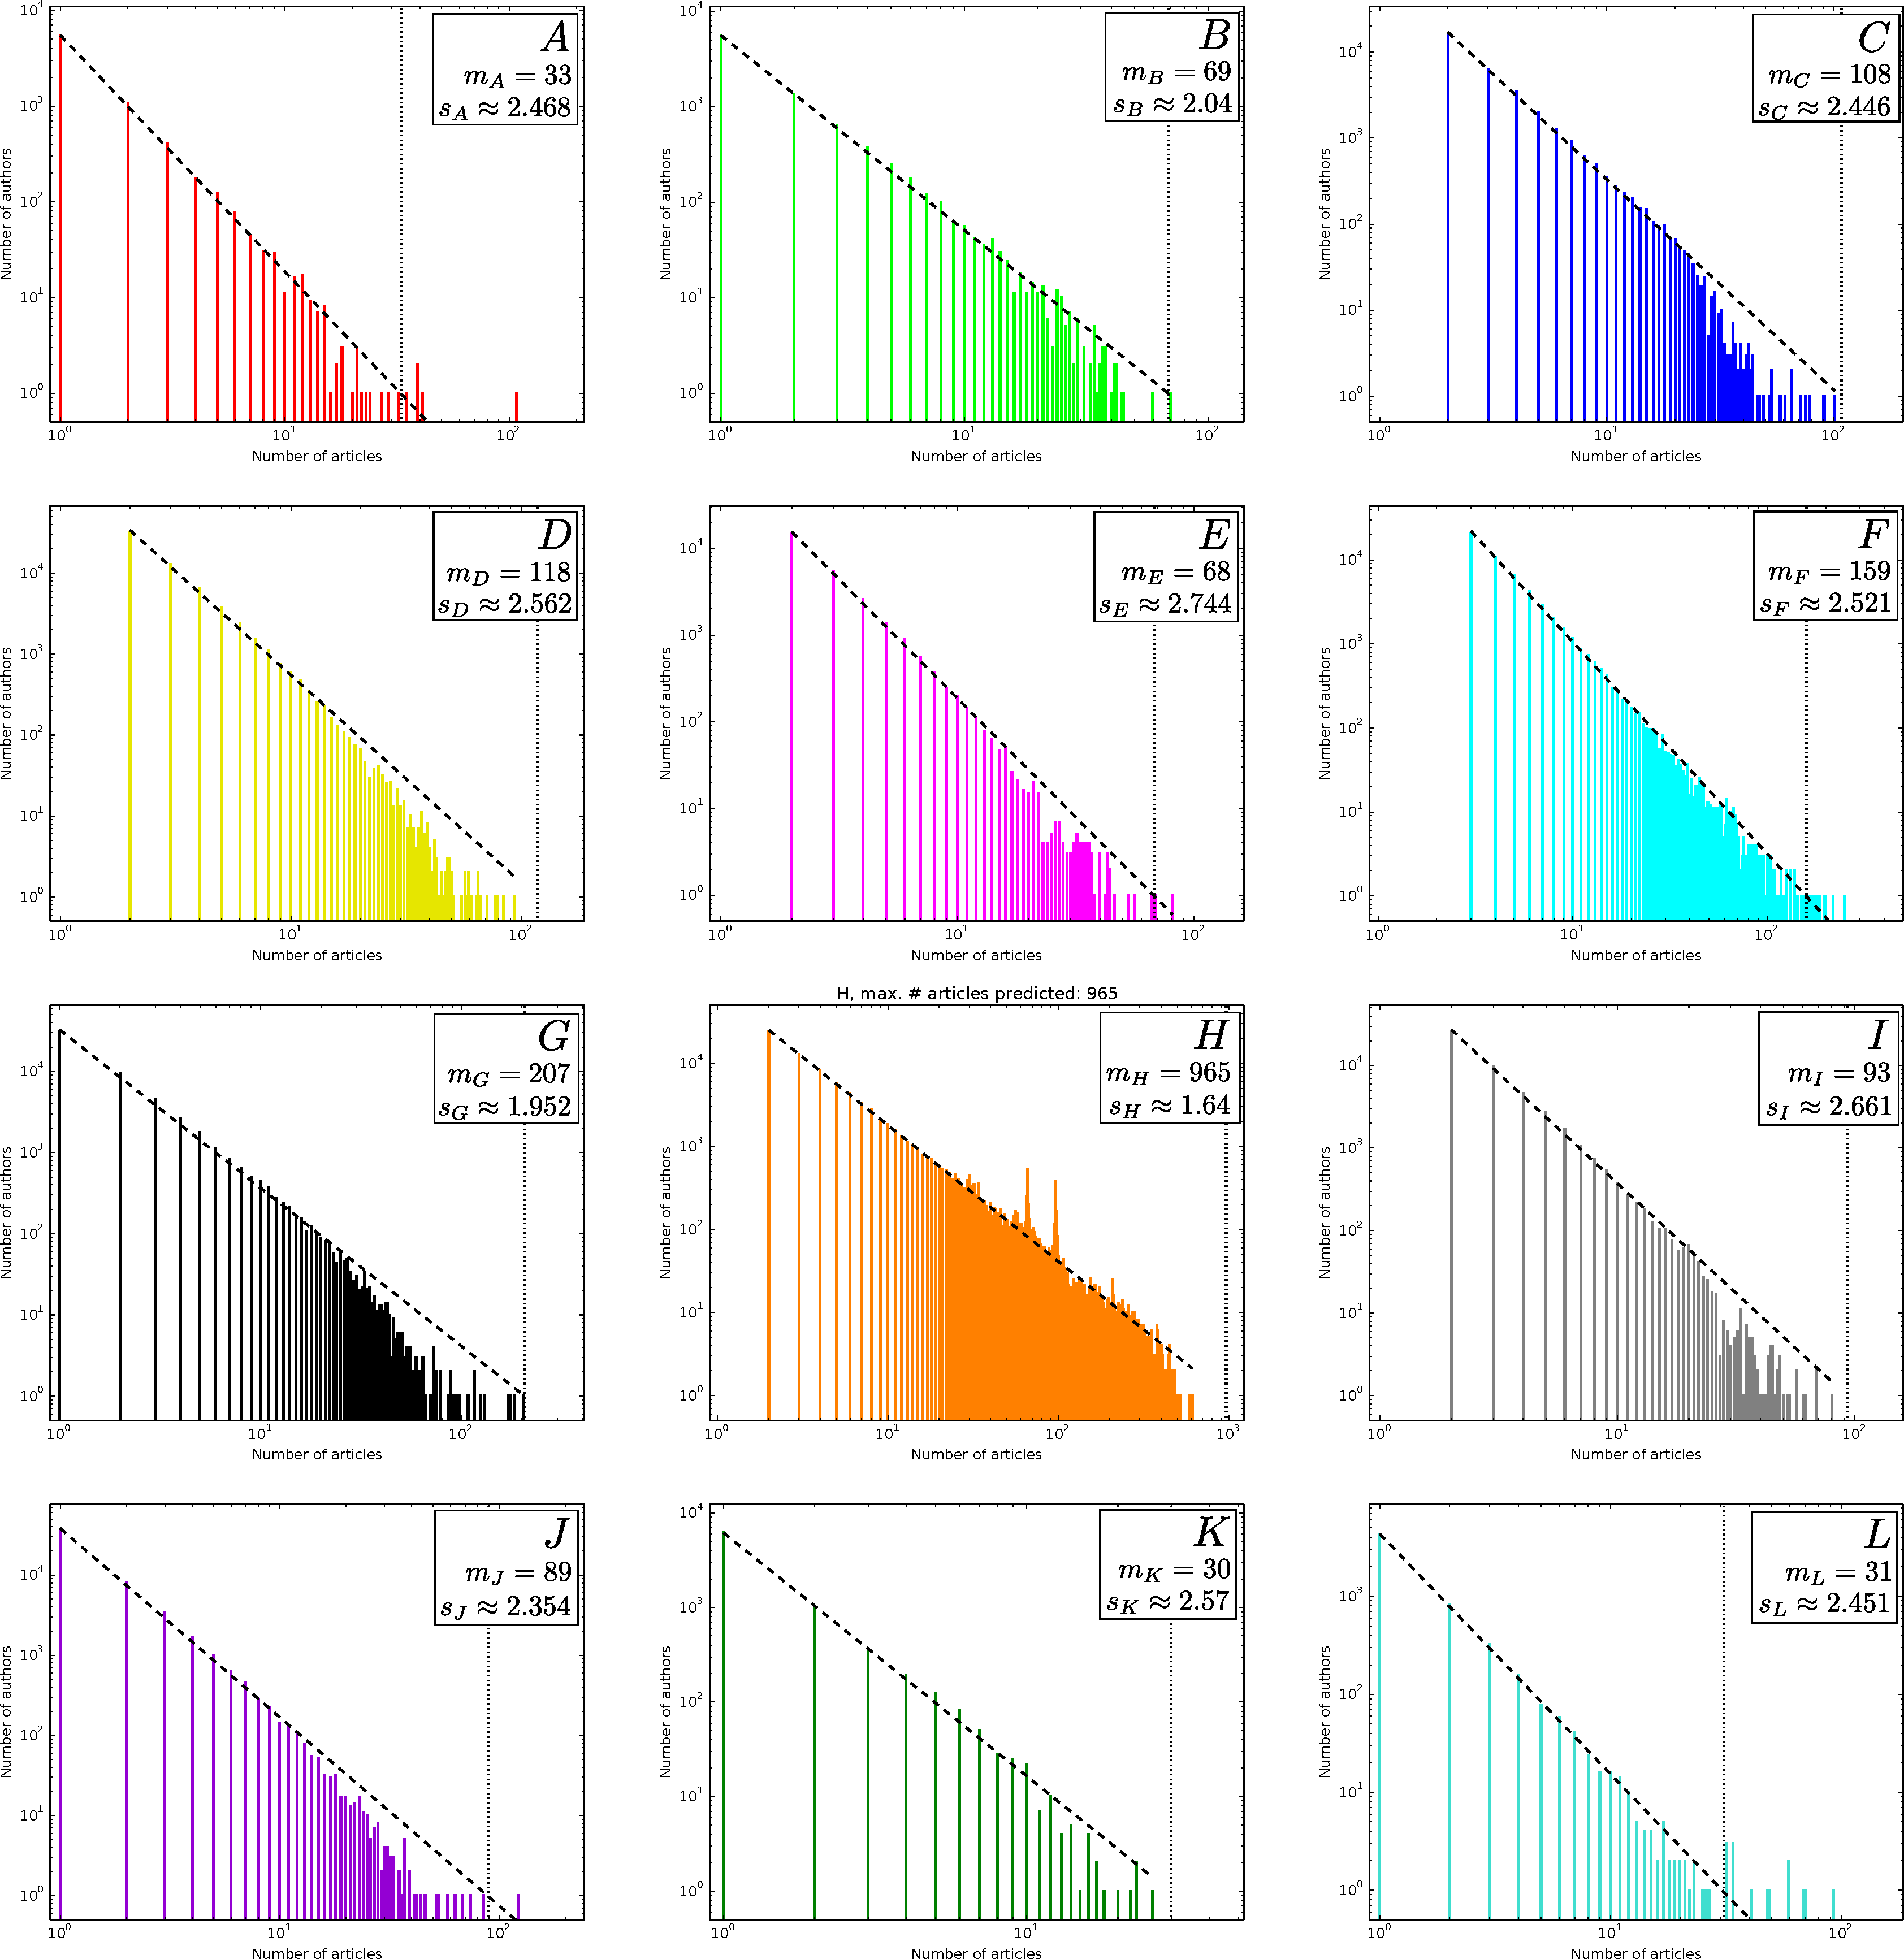
\includegraphics[width=\textwidth]{../figures/ABCDEFGHIJKL.pdf}
 \caption{Blah...}
 \label{fig:1}
\end{figure*}

\section{Methodology}
We consider an arbitrary selection of 12 journals, labelled by capital letters, ${\cal J}=\{A,B,C,D,E,F,G,H,I,J,K,L\}$, available on the Web of Science database~\cite{WoS}. 

\paragraph{}
{\bf Remark.}\textit{
Each element of ${\cal J}$ corresponds to a peer-reviewed journal with a significant number of publications within the last decades. 
We do not explicitly give the journals' names for privacy reasons.
}

\paragraph{}
Within each journal $j\in {\cal J}$, we count the number $n^j_i$ of articles published by author $i$, which gives the set of data $\{n^j_i\}$. 
From these data, we can the compute 
\begin{align}
 a_j(n)\coloneqq\#\{i\colon n^j_i = n\}\, ,
\end{align}
which are represented in logarithmic scales in Fig.~\ref{fig:1}, for each journal. 
We then fit a power law (black dashed lines in Fig.~\ref{fig:1}) to the data of each journal $j\in{\cal J}$. 
The exponent $s_j$ of the power law 
\begin{align}
 z_j(n) &= C_jn^{-s_j}
\end{align}
is obtained by a maximum likelihood estimator, following~\cite{Cla09}, and $C_j$ is the constant normalizing the distribution. 
Finally, we compute the theoretical maximum number of articles, $m_j$, which is the value satisfying $N_jz_j(m_j)\approx1$, where $N_j$ is the total number of articles published in journal $j$. 

\paragraph{}
{\bf Remark.}\textit{
 We restricted our investigation to publications labelled as ``Article'' in the WoS database.
 For some journals, the number of authors was too large to be downloaded from the Web of Science database. 
 As a consequence, some authors having published only one or two articles in these journals had to be removed from the data. 
 As this might influence our results, we indicate when this was the case in the captions. 
 Note also that we did not take into account articles published anonymously. 
 \textcolor{red}{Do the same for the time-splitted data !!!}
}

\section{Results}
To the eye, the histograms for all journals considered follow a power law, also called a Zipf's law for discrete-valued variables. 
The error of the fit is plotted in Fig.~\textcolor{red}{Figure}, confirming that Zipf's law correctly describes the distribution of $N^j_k$. 

The Zipf's law  approximates the data well, slightly overestimating it for large values of $n$. 


\paragraph{}
{\bf General explanation. }
Our explanation to this fact is that the evolution of the number of articles in a journal is described by a \emph{preferential attachment} process. 
In other words, it means the probability that a new article published in a given journal 
is signed by an author is proportional to the number of articles published by this author in the given journal. 
Heuristically, our argument is that if an author published a lot of article in a journal, it means (i) that they write a lot of papers, 
and (ii) that their research topic is well-aligned with the topics covered by the journal. 
Consequences (i) and (ii) together imply that this author is likely to published again in this journal. 

To make this more rigorous, compared for \textcolor{red}{two} journals the number of authors having published $k$ articles at time $t$ 
with the number of articles published by these authors between times $t$ and $t+1$. 
Defining $m_k(t,s)$ as the number of articles published between $t$ and $s$ by the authors with $k$ articles at time $t$, we plot in Fig.~\textcolor{red}{Figure} the values of 
$m_k(t,t+1)/N_k(t)$ with respect to $k$ for years $t\in\{1999,...,2008\}$. 
These values have a linear correlation coefficient of \textcolor{red}{BLAH}, supporting a fairly good linear dependence, 
\begin{align}
 m_k(t,t+1) &\approx k\cdot N_k(t)\, . 
\end{align}
\textcolor{red}{Restrict the data to a time span of max. 30 years to remove authors who are not publishing anymore.}

\begin{figure*}
 \centering
 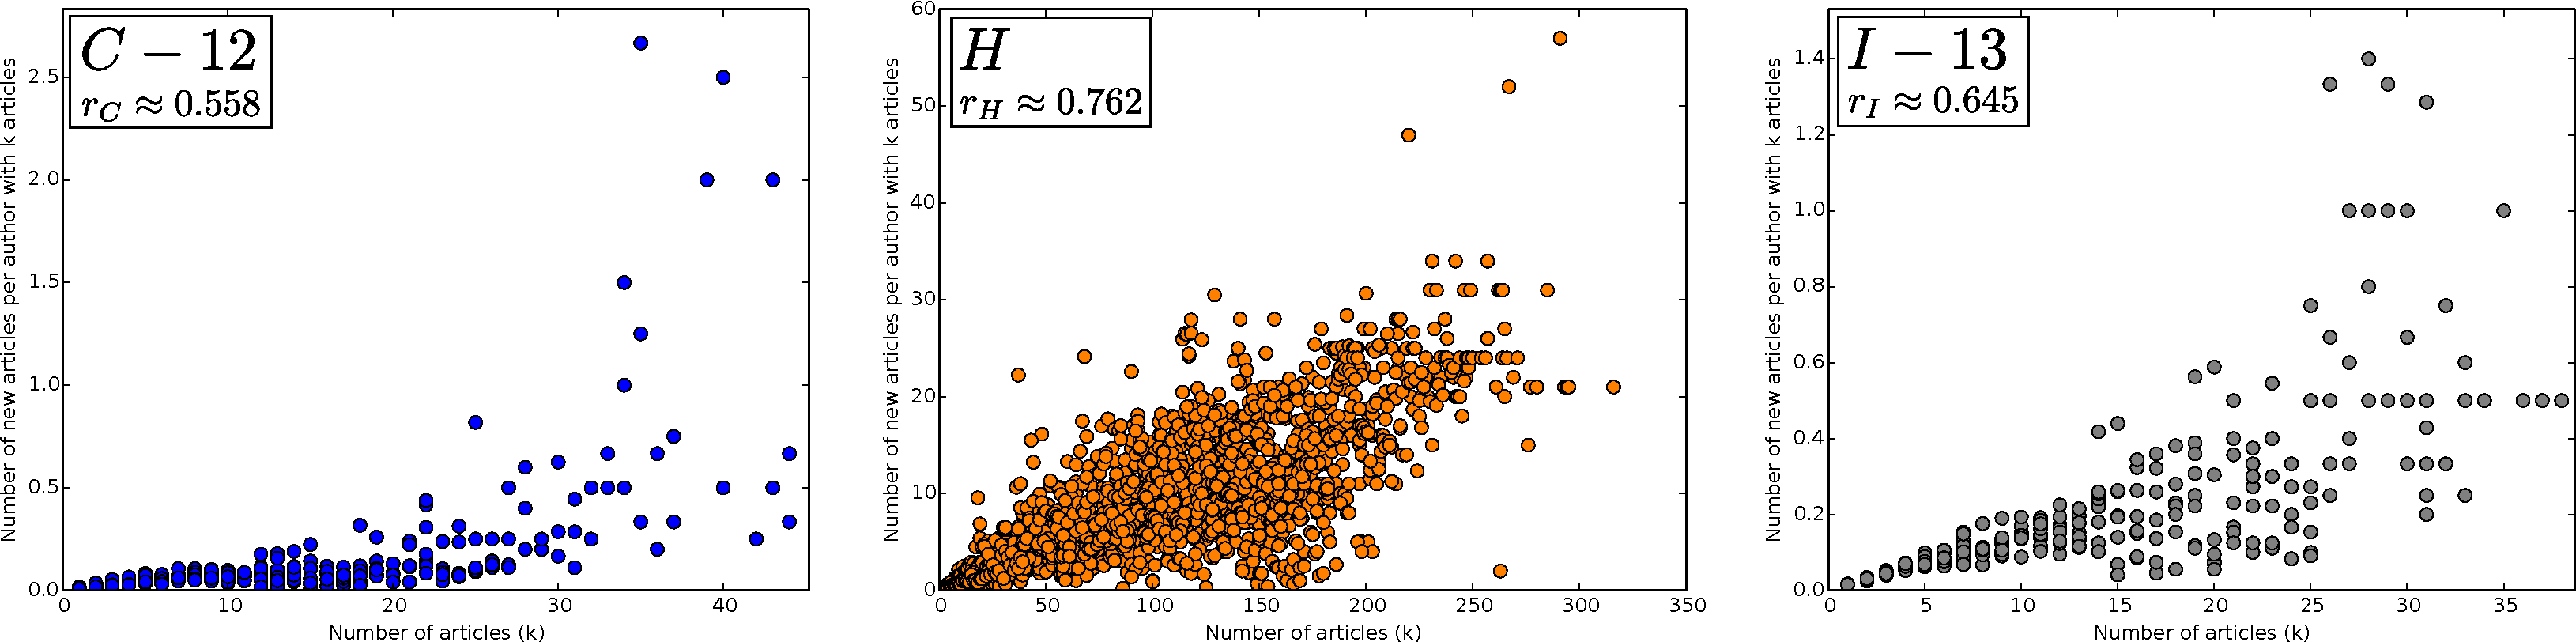
\includegraphics[width=\textwidth]{../figures/CHI_correl.pdf}
 \caption{Blih...}
 \label{fig:2}
\end{figure*}


The probability that a new paper is signed by an author with $k$ publications is then proportional to $k$. 
The dynamics of the number of authors with $k$ articles is then described by Eq.~(1) in~\cite{Kra00}, with exponent $\gamma\approx 1$. 
According to~\cite{Kra00}, after a long enough time, the distribution of $N_k$ follows a power law, which agrees with our observations.

\paragraph{}
{\bf Exceptions. }
The general distribution of the number of authors with respect to the number of paper per author is quite clear in our analysis. 
However, in some journals, we observe anomalies (\textcolor{red}{see Figs...}). 
It appears that sometimes, some authors publish more articles in a journal than what our Zipf's law distribution would predict. 
These authors, who we refer to as \emph{K-players}, are supposedly some very influencial scientists in the journal considered here, and they literally \emph{beat the power law}.

\paragraph{}
{\bf Remark.}\textit{
We emphasize that we checked that these K-players are not artifacts due to multiple authors having the same name which would count as the same person. 
In all cases presented here, there is a unique person appearing in the authors' list of a very large number of papers. 
}

\section{Conclusion}
The aim of this letter is to point out some puzzling observations that could lead to further investigations. 
Our investigation are limited to a rather small number of journals and would need a large scale study to confirm the general validity of this power law behavior. 
However, in our opinion, the regularity of our observations regardless of the size and age of the journal, 
as well as with respect of the time interval considered are sufficient evidence to formulate a conjecture. 


\bibliographystyle{pnas-new}
\bibliography{bibliography}

\end{document}
